\chapter{Results and Analysis}
\section{Signal Characteristics}
In order to understand the nature of the problem there was requirment for pre-analysis of data. The primary dataset used is 2 seconds of electric field recordings, from a particular instance of exceedingly high lightning activity. This raw data was recorded with a sampling frequency $f_s = 1\si{\mega\hertz}$. These are broadband recordings, the time series is shown by Figure \ref{fig:realData} and the frequency spectrum of the recording is shown by the Figure \ref{fig:realFFT} shows that they cover the band of 0-300\si{\kilo\hertz}. The large spike at 198kHz is Radio 4's long wave service, this is an AM transmission hence it needs to have a very large amplitude to avoid background interference. Unlike the VLF signals we are interested in which are phase/frequency modulated, therefore the transmitted power lower.


\begin{figure}[h!]
    \begin{subfigure}[b]{0.5\textwidth}
        \centering
        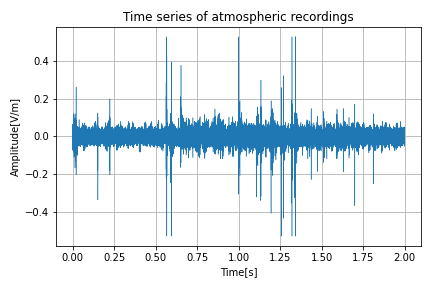
\includegraphics[width = \textwidth]{figs/sig_character/timeseries.png}
        \caption{Time Series}
        \label{fig:realData}
    \end{subfigure}
    \begin{subfigure}[b]{0.5\textwidth}
    `   \centering
        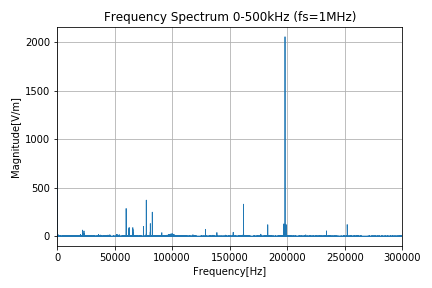
\includegraphics[width = \textwidth]{figs/sig_character/fft_data.png}
        \caption{FFT}
        \label{fig:realFFT}
    \end{subfigure}
    \caption{Unfiltered Real Data}
\end{figure}

Figure \ref{fig:vlfspect} is a spectrogram showing the band of interest to this problem and effectively represents the problem space. It can be seen in this plot that the vertical lines represent active transmitters of which there are five. The horizontal lines represent interference events. Figure \ref{fig:transSpect} shows the more localised contained the centre frequencies of the transmitters visible. This clearly illustrates the impulsive nature of noise, in this plot there are 4 visible impulses, the cause of which is the electromagnetic radiation produced by a lightening event. 

\begin{figure}[h!]
        \centering
        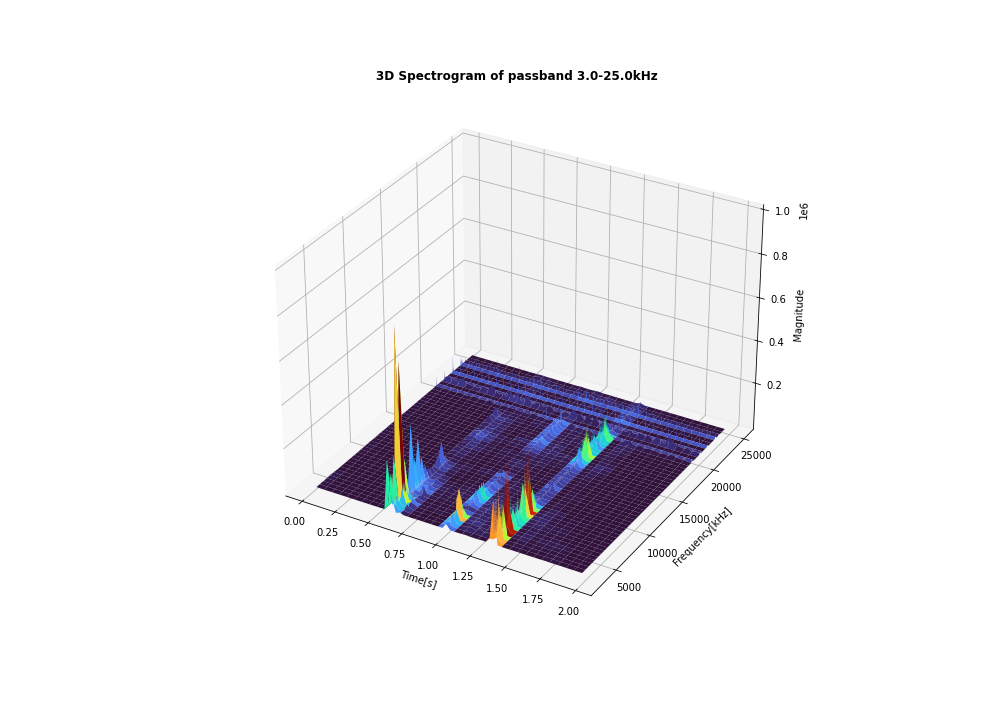
\includegraphics[width = \textwidth]{figs/sig_character/vlfspectrogram.png}
        \caption{3D spectrogram covering VLF band}
        \label{fig:vlfspect}
\end{figure}
\begin{figure}[h!]
        \centering
        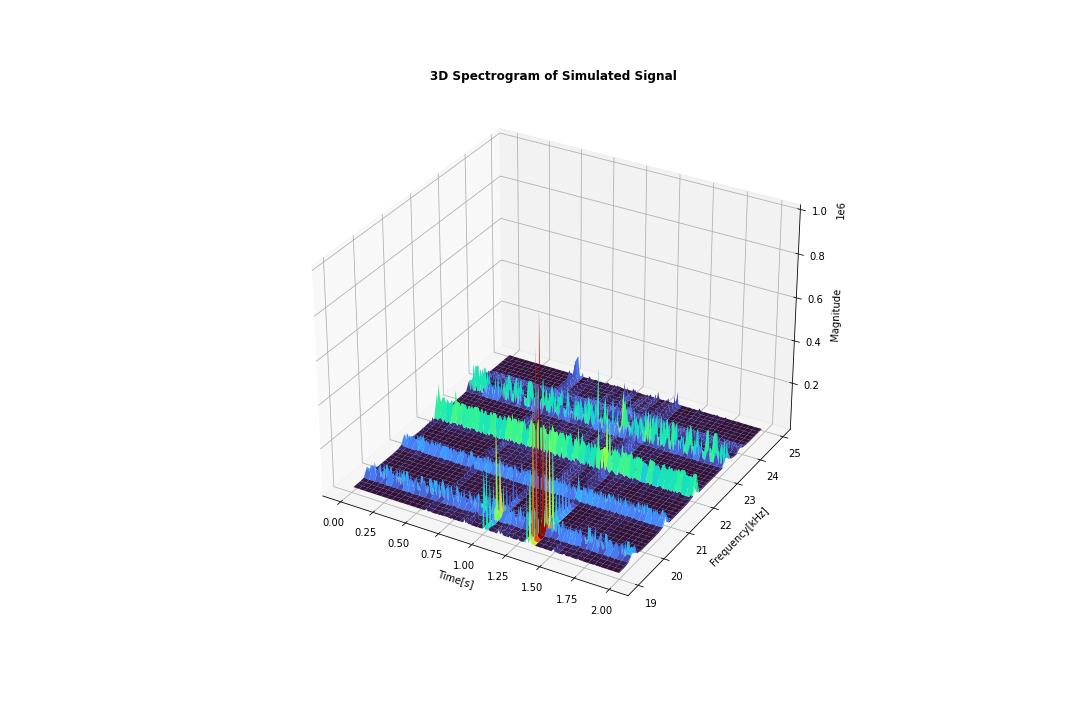
\includegraphics[width = \textwidth]{figs/sig_character/transmitters_spectrogram.png}
        \caption{Band containing active transmitters}
        \label{fig:transSpect}
\end{figure}

Figure \ref{fig:absAmplitude} shows the absolute amplitude of the five active transmitters that are in the recorded dataset. Additionally as described in section \ref{sec:investigations} the plots also show the limits used for noise bounding in order to estimate the noise signal for this example. $k=1.5$ has been used in order to set this limit. These properties are then used to calculate the noise signal and then in turn estimate to the Signal to Noise ratio. This estimate is calculated and shown by table \ref{tab:snr1}. By referring back to figure \ref{fig:transSpect} in addition to the amplitude plots, the spikier the plots are can justify the inference that there is much more interference present in the signal. 

\begin{figure}[h!]
    \centering
    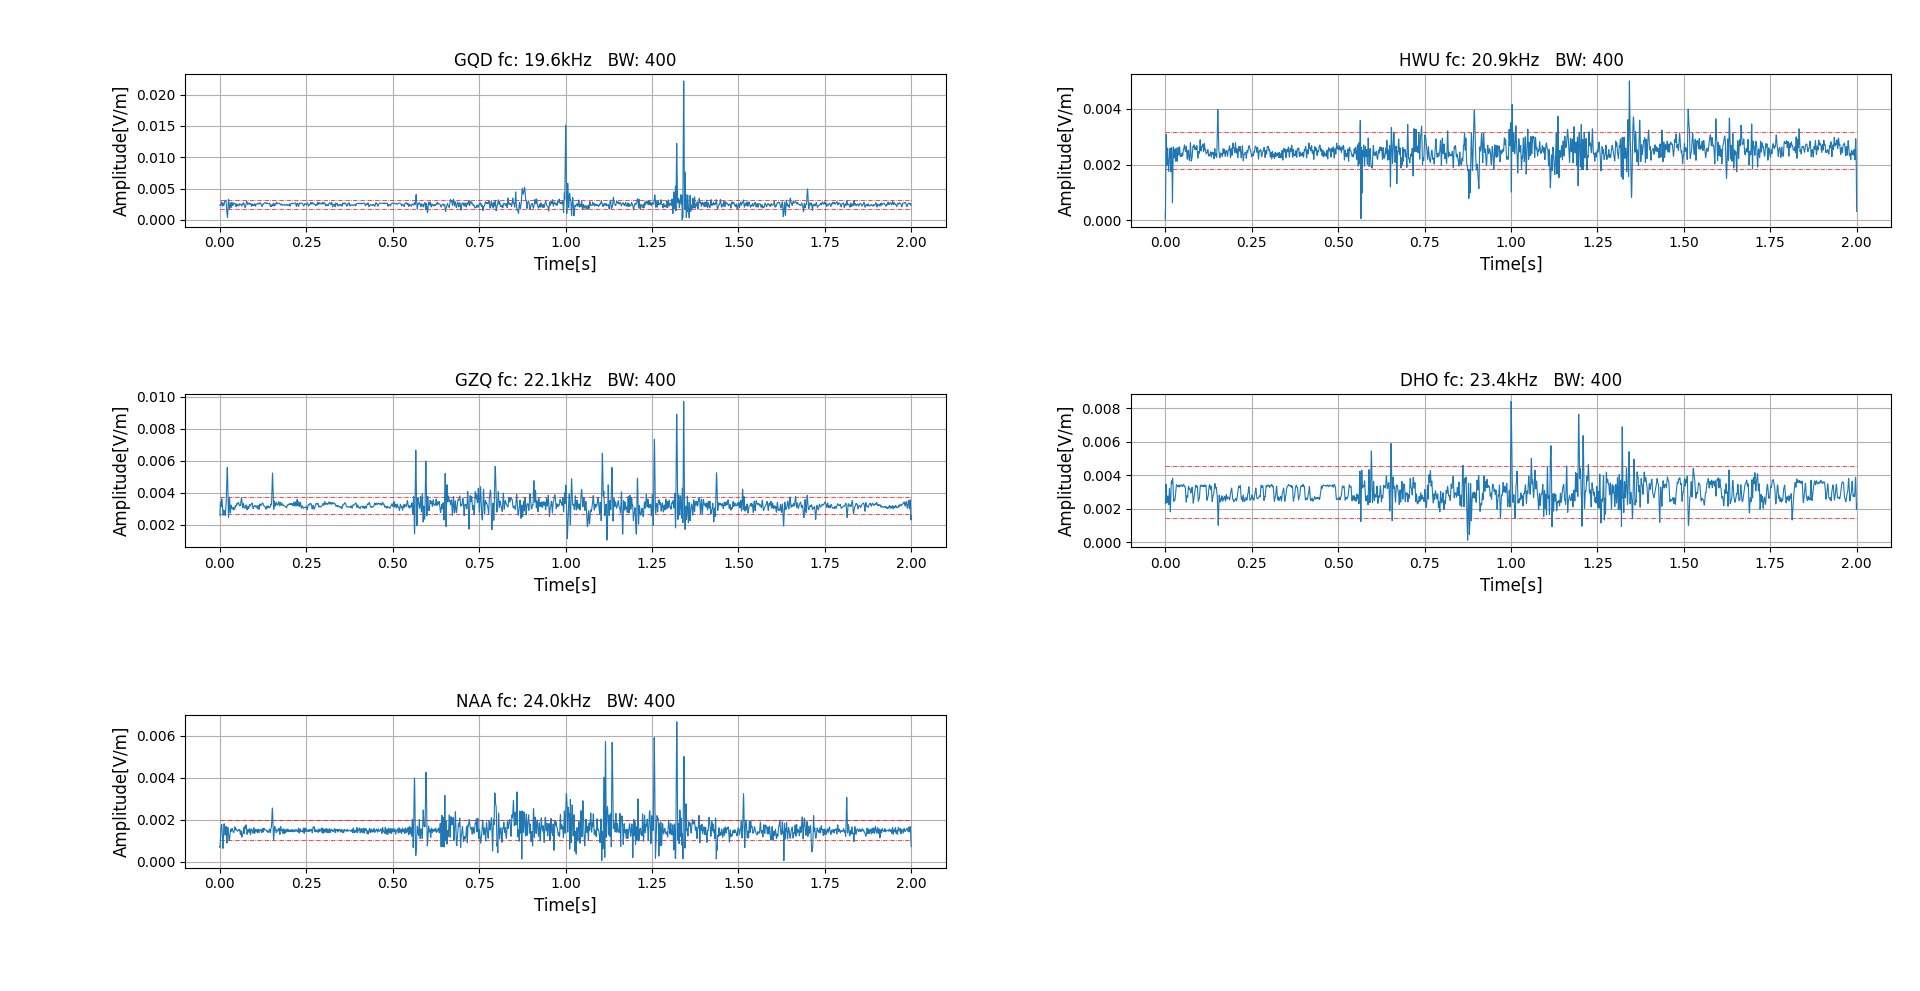
\includegraphics[width = \textwidth]{figs/sig_character/abs_amplitude.png}
    \caption{\centering Absolute Amplitude of Complex Trace of VLF Transmitters, shown with upper and lower limits for noise bounding.}
    \label{fig:absAmplitude}
\end{figure}

\begin{table}[h!]
\centering
    \begin{tabular}{l|l|l}
    Callsign & SNR [dB] & Centre Frequency $f_c$ [kHz] \\
    \hline
    GQD & 17.2 & 19.6 \\
    HWU & 62.6 & 20.9 \\
    GZQ & 36.1 & 22.1 \\
    DHO38 & 35.4 & 23.4 \\
    NAA & 20.64 & 24
    \end{tabular}
\caption{Estimated Signal to Noise ratio of VLF transmitters}
\label{tab:snr1}
\end{table}

Appendix X contains the figures related to the demodulated signals for each transmitter, as it is clear that MSK is used as the modulation technique illustrated by the constant frequency for each symbol, the gradient changes sign when the symbol changes. This represent a zero crossing in the first differential which corresponds to the instantaneous frequency.
\pagebreak
\section{Simulation}
\subsection{Control Signal}
The development of a successful simulation was key in order to assess the problem as previously explained the MSK signal consists of an inphase and quadrature component, these are cosine and sine waves amplitude modulated with the pulse shaped baseband signal. This is shown by figure \ref{fig:carrier}, which shows these signals. They are then combined in order to create the final signal that is suitable for transmission. The final complex waveform is shown by figure \ref{fig:3DBB}, where the symbol switch point can be seen. The baseband frequency is determined by the bitrate, which is $f_{1bb} = \frac{1}{T_b}$. This means that in theory there is potential for a bit change everytime there is an axis crossing, in reality this is eight points where the direction of the phasor can change either side of the axis, depending on which direction the phasor is moving depends on which one of these points it will switch.

\begin{figure}[h!]
    \centering
    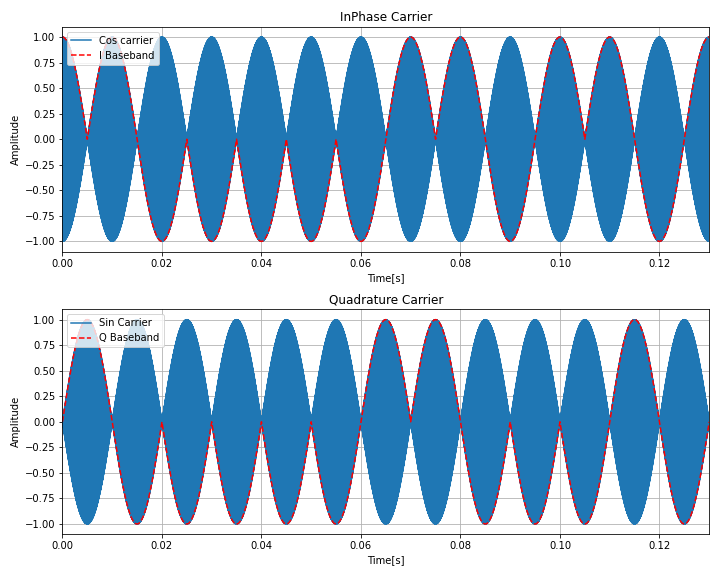
\includegraphics[width = \textwidth]{figs/sim/carrier.png}
    \caption{\centering Amplitude Modulated Cos and Sin carriers carresponding to Inphase and Quadrature elements}
    \label{fig:carrier}
\end{figure}
\begin{figure}[h!]
    \centering
    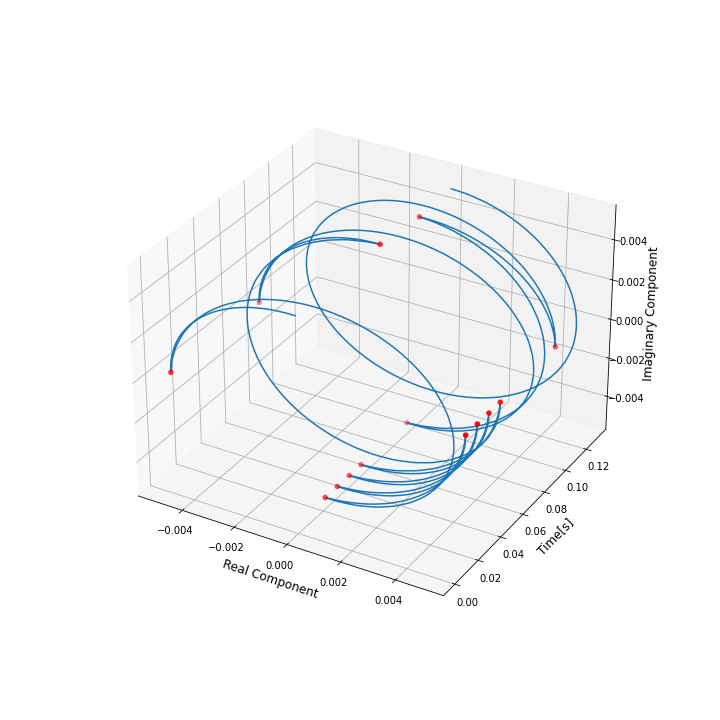
\includegraphics[height = \textwidth]{figs/sim/3dbaseband.png}
    \caption{3D Baseband Plot. \small{Red Markers highlight symbol changes}}
    \label{fig:3DBB}
    \caption{Development of MSK simulation}
\end{figure}

\subsection{Additive Noise}